\setlength{\LTpre}{\baselineskip}
\setlength{\LTpost}{6pt}
\small
\renewcommand{\arraystretch}{1.1}
\setlength{\tabcolsep}{3pt}
\begin{longtable}{C{3.4cm}C{3.7cm}C{7.0cm}}
\caption{Compostos selecionados para prospecção.}\label{tab:ligantes_spe_metodos}\\
\toprule Ligante & Estrutura bidimensional & Fonte da estrutura ou referência \\
\midrule
\endfirsthead
\multicolumn{3}{c}{\tablename~\thetable\ (continuação)}\\
\toprule Ligante & Estrutura bidimensional & Fonte da estrutura ou referência \\
\midrule
\endhead
\midrule
\multicolumn{3}{r}{Continua na próxima página}\\
\endfoot
\bottomrule
\endlastfoot
Ácido ferúlico & 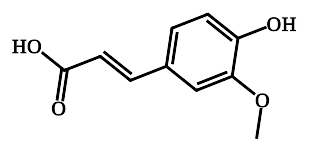
\includegraphics[width=3.2cm,height=0.9cm,keepaspectratio]{image/estruturas_ligantes_integracao/miniaturas/spe_Acido_Ferulico.png} & Extrato de biomassa de \textit{T. tetrahele} \parencite{mai2026} \\
Ácido galacturônico & 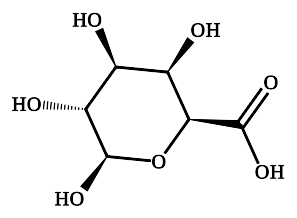
\includegraphics[width=3.2cm,height=0.9cm,keepaspectratio]{image/estruturas_ligantes_integracao/miniaturas/spe_Acido_Galacturonico.png} & Exopolissacarídeos de \textit{T. suecica} \parencite{parra2020} \\
Ácido gálico & 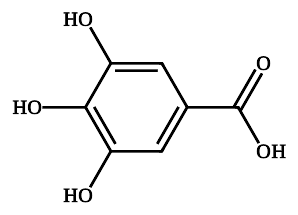
\includegraphics[width=3.2cm,height=0.9cm,keepaspectratio]{image/estruturas_ligantes_integracao/miniaturas/spe_Acido_Galico.png} & Extrato de biomassa de \textit{T. tetrahele} \parencite{mai2026} \\
Ácido glucurônico & 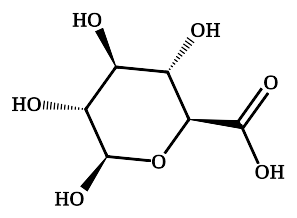
\includegraphics[width=3.2cm,height=0.9cm,keepaspectratio]{image/estruturas_ligantes_integracao/miniaturas/spe_Acido_Glucuronico.png} & Exopolissacarídeos de \textit{T. suecica} \parencite{parra2020} \\
D-Galactose & 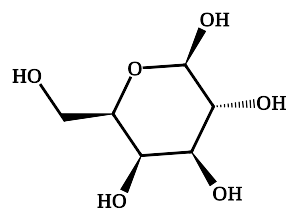
\includegraphics[width=3.2cm,height=0.9cm,keepaspectratio]{image/estruturas_ligantes_integracao/miniaturas/spe_D_Galactose.png} & Biomassa de \textit{T. chuii}; exopolissacarídeos de \textit{T. suecica} \parencite{brown1991,pereira2019,parra2020} \\
D-Glicose & 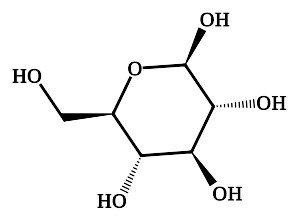
\includegraphics[width=3.2cm,height=0.9cm,keepaspectratio]{image/estruturas_ligantes_integracao/miniaturas/spe_D_Glicose.png} & Biomassa de \textit{T. chuii}; exopolissacarídeos de \textit{T. suecica} \parencite{brown1991,pereira2019,parra2020} \\
D-Gulose & 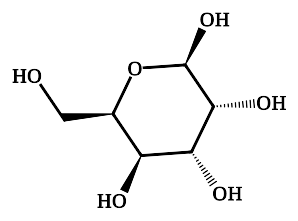
\includegraphics[width=3.2cm,height=0.9cm,keepaspectratio]{image/estruturas_ligantes_integracao/miniaturas/spe_D_Gulose_Raro_presente_na_SPE.png} & Parede celular de \textit{T. striata} \parencite{becker1989} \\
D-Manose & 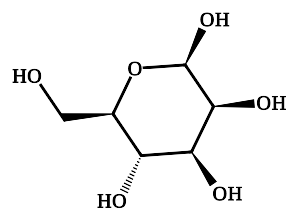
\includegraphics[width=3.2cm,height=0.9cm,keepaspectratio]{image/estruturas_ligantes_integracao/miniaturas/spe_D_Manose.png} & Biomassa de \textit{T. chuii}; exopolissacarídeos de \textit{T. suecica} \parencite{brown1991,pereira2019,parra2020} \\
D-Xilose & 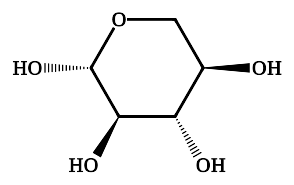
\includegraphics[width=3.2cm,height=0.9cm,keepaspectratio]{image/estruturas_ligantes_integracao/miniaturas/spe_D_Xilose.png} & Exopolissacarídeos de \textit{T. suecica} \parencite{parra2020} \\
\textit{Dha} & 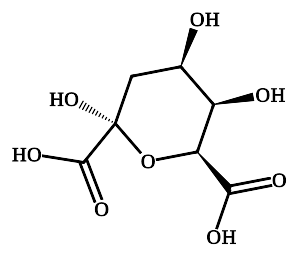
\includegraphics[width=3.2cm,height=0.9cm,keepaspectratio]{image/estruturas_ligantes_integracao/miniaturas/spe_Dha_3_deoxy_D_lyxo_hept_2_ulopyranosaric_acid.png} & Parede celular de \textit{T. striata} \parencite{becker1989} \\
Galactose-6-sulfato & 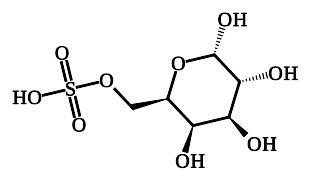
\includegraphics[width=3.2cm,height=0.9cm,keepaspectratio]{image/estruturas_ligantes_integracao/miniaturas/spe_Galactose_6_sulfato.png} & Comparador estrutural em galactanos de algas vermelhas (\textit{Gloiopeltis} e \textit{Acanthophora}); ocorrência em \textit{Tetraselmis} não identificada \parencite{tuvikene2015funorans,duarte2004} \\
Glicose-6-sulfato & 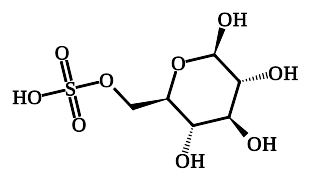
\includegraphics[width=3.2cm,height=0.9cm,keepaspectratio]{image/estruturas_ligantes_integracao/miniaturas/spe_Glicose_6_sulfato.png} & Em polissacarídeo sulfatado de \textit{T. suecica}, a sulfatação foi proposta no O-6 de resíduos de glicose \parencite{li2026tetraselmis} \\
KDO & 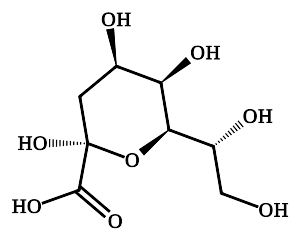
\includegraphics[width=3.2cm,height=0.9cm,keepaspectratio]{image/estruturas_ligantes_integracao/miniaturas/spe_KDO_3_deoxy_D_manno_oct_2_ulosonic_acid.png} & Parede celular de \textit{T. striata} \parencite{becker1989} \\
L-Arabinose & 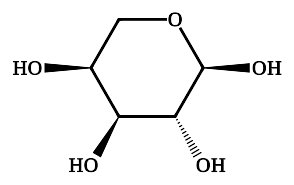
\includegraphics[width=3.2cm,height=0.9cm,keepaspectratio]{image/estruturas_ligantes_integracao/miniaturas/spe_L_Arabinose.png} & Biomassa de \textit{T. chuii}; exopolissacarídeos de \textit{T. suecica} \parencite{brown1991,pereira2019,parra2020} \\
L-Fucose & 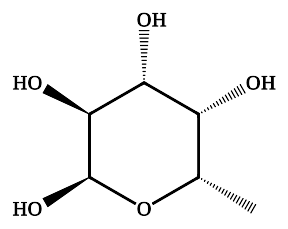
\includegraphics[width=3.2cm,height=0.9cm,keepaspectratio]{image/estruturas_ligantes_integracao/miniaturas/spe_L_Fucose.png} & Exopolissacarídeos de \textit{T. suecica} \parencite{parra2020} \\
L-Ramnose & 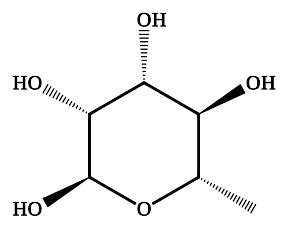
\includegraphics[width=3.2cm,height=0.9cm,keepaspectratio]{image/estruturas_ligantes_integracao/miniaturas/spe_L_Ramnose.png} & Biomassa de \textit{T. chuii}; exopolissacarídeos de \textit{T. suecica} \parencite{brown1991,pereira2019,parra2020} \\
$\alpha$-Kdo & 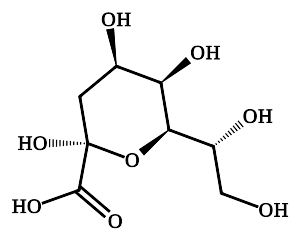
\includegraphics[width=3.2cm,height=0.9cm,keepaspectratio]{image/estruturas_ligantes_integracao/miniaturas/spe_alpha_Kdo_Isomero_comum_em_polissacarideos.png} & Comparador estrutural; sem fonte de ocorrência identificada \\
\end{longtable}
\normalsize
\renewcommand{\arraystretch}{1.25}
\setlength{\tabcolsep}{6pt}
